\begin{figure}[H]
\centering
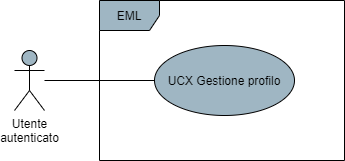
\includegraphics[scale=0.6]{res/UseCase/Immagini/ProfiloGenerale}
\caption{Diagramma UML per modulo del profilo}
\end{figure}

\subsubsection{UCX - Gestione profilo}
\begin{itemize}
\item \textbf{Attori primari}: cliente;
\item \textbf{Descrizione}: per gli utenti autenticati come clienti è disponibile una pagina del profilo in cui è possibile gestire i dati personali e visualizzare gli ordini effettuati.
\item \textbf{Scenario Principale}: il cliente accede alla pagina del profilo personale ed ha a disposizione le seguenti funzionalità:
\begin{itemize}
\item Visualizzazione dati del profilo (\textbf{UCX.1});
\item Modifica dati del profilo (\textbf{UCX.2});
\item Visualizzazione ordini effettuati dall'utente (\textbf{UCX.3});
\item Eliminazione profilo (\textbf{UCX.4}).
\end{itemize}
\item \textbf{Precondizione}: l'utente è autenticato come cliente nel sito e ha a disposizione la pagina del profilo;
\item \textbf{Postcondizione}: l'utente visualizza la pagina del profilo ed ha accesso a varie funzionalità.
\end{itemize}

\begin{figure}[H]
\centering
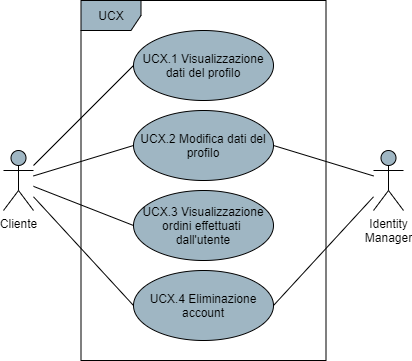
\includegraphics[scale=0.6]{res/UseCase/Immagini/GestioneProfilo}
\caption{Diagramma UML per UCX - Gestione profilo}
\end{figure}

\subsubsection{UCX.1 - Visualizzazione dati del profilo}
\begin{itemize}
\item \textbf{Attori primari}: cliente;
\item \textbf{Descrizione}: il cliente visualizza i suoi dati personali presenti nel sistema;
\item \textbf{Scenario Principale}: il cliente si trova nella pagina del profilo e visualizza i seguenti dati personali:
\begin{itemize}
\item Nome;
\item Cognome;
\item Indirizzo di fatturazione;
\item Email.
\end{itemize}
\item \textbf{Precondizione}: il cliente si trova nella pagina del profilo;
\item \textbf{Postcondizione}: vengono visualizzati i dati personali del cliente.
\end{itemize}

\subsubsection{UCX.2 - Modifica dati del profilo}
\begin{itemize}
\item \textbf{Attori primari}: utente generico;
\item \textbf{Attori secondari}: Identity Manager;
\item \textbf{Descrizione}: il cliente può modificare i dati personali presenti nella sua pagina del profilo;
\item \textbf{Scenario Principale}: il cliente si trova nella pagina del profilo e clicca un tasto dedicato per andare nella pagina di modifica, in cui sono presenti dei campi modificabili già compilati con i valori attuali. Una volta che i campi hanno al suo interno i valori previsti dal cliente, è possibile continuare con il salvataggio dei dati da parte del sistema;
\item \textbf{Precondizione}: il cliente si trova nella pagina del profilo;
\item \textbf{Postcondizione}: vengono modificati i dati personali del cliente presenti nel profilo in base alle sue intenzioni.
\end{itemize}

\subsubsection{UCX.3 - Visualizzazione ordini effettuati dall'utente}
\begin{itemize}
\item \textbf{Attori primari}:
\item \textbf{Attori secondari}:
\item \textbf{Descrizione}:
\item \textbf{Scenario Principale}:
\item \textbf{Estensioni}:
\item \textbf{Specializzazioni}:
\item \textbf{Precondizione}:
\item \textbf{Postcondizione}:
\end{itemize}

\begin{figure}[H]
\centering
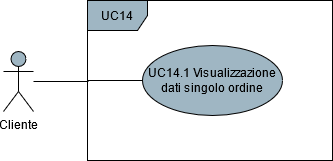
\includegraphics[scale=0.6]{res/UseCase/Immagini/VisualizzazioneOrdini}
\caption{Diagramma UML per UCX.3 - Visualizzazione ordini effettuati dall'utente}
\end{figure}

\subsubsection{UCX.3.1 - Visualizzazione dati singolo ordine}
\begin{itemize}
\item \textbf{Attori primari}:
\item \textbf{Attori secondari}:
\item \textbf{Descrizione}:
\item \textbf{Scenario Principale}:
\item \textbf{Estensioni}:
\item \textbf{Specializzazioni}:
\item \textbf{Precondizione}:
\item \textbf{Postcondizione}:
\end{itemize}

\subsubsection{UCX.4 - Eliminazione profilo}
\begin{itemize}
\item \textbf{Attori primari}:
\item \textbf{Attori secondari}:
\item \textbf{Descrizione}:
\item \textbf{Scenario Principale}:
\item \textbf{Estensioni}:
\item \textbf{Specializzazioni}:
\item \textbf{Precondizione}:
\item \textbf{Postcondizione}:
\end{itemize}
